\documentclass[11pt,spanish]{endm}
\usepackage{endmmacro}
\usepackage{graphicx}
\usepackage[spanish]{babel}
\selectlanguage{spanish}
\usepackage[utf8]{inputenc}
\usepackage{caption}
\usepackage{subcaption}
\usepackage{dsfont}


% The following is enclosed to allow easy detection of differences in
% ascii coding.
% Upper-case    A B C D E F G H I J K L M N O P Q R S T U V W X Y Z
% Lower-case    a b c d e f g h i j k l m n o p q r s t u v w x y z
% Digits        0 1 2 3 4 5 6 7 8 9
% Exclamation   !           Double quote "          Hash (number) #
% Dollar        $           Percent      %          Ampersand     &
% Acute accent  '           Left paren   (          Right paren   )
% Asterisk      *           Plus         +          Comma         ,
% Minus         -           Point        .          Solidus       /
% Colon         :           Semicolon    ;          Less than     <
% Equals        =           Greater than >          Question mark ?
% At            @           Left bracket [          Backslash     \
% Right bracket ]           Circumflex   ^          Underscore    _
% Grave accent  `           Left brace   {          Vertical bar  |
% Right brace   }           Tilde        ~
\usepackage{adjustbox} % Used to constrain images to a maximum size
\newcommand{\Nat}{{\mathbb N}}
\newcommand{\Real}{{\mathbb R}}
\def\lastname{Please list your Lastname here}

\begin{document}

% DO NOT REMOVE: Creates space for Elsevier logo, ScienceDirect logo
% and ENDM logo
\begin{verbatim}
\end{verbatim}\vspace{2.5cm}

\begin{frontmatter}

\title{Métodos Númericos}

%\subtitle{\tituloTP}{Trabajo Práctico Nro. 3}
%\subtitle{\subTituloTP}{\emph{Cuadrados Mínimos Lineales}}

\author{Catriel Omar D'Elía\thanksref{myemail}}
\author{Gian Franco Lancioni\thanksref{myemail1}}
\author{Joaquín Perez Centeno\thanksref{myemail2}}
\address{Depatamento de Computación\\ Universidad de Buenos Aires\\ Buenos Aires, Argentina}

\thanks[myemail]{Email:
   \href{catriel.delia@gmail.com} {\texttt{\normalshape
   catriel.delia@gmail.com}}} \thanks[myemail1]{Email:
   \href{gianflancioni@gmail.com} {\texttt{\normalshape
   gianflancioni@gmail.com}}} \thanks[myemail2]{Email:
   \href{joaquinpcenteno@gmail.com} {\texttt{\normalshape
   joaquinpcenteno@gmail.com}}}

%\section {Resúmen}

\begin{abstract}
  En este trabajo práctico se analizará el retraso de vuelos,
  aplicando técnicas de \textbf{\textit{Métodos Numéricos}}\ y
  \textbf{\textit{Data Science,}}\ en particular
  \textbf{\textit{Regresiones Lineales de Cuadrados Mínimos}}\ sobre
  un conjunto de datos con el objetivo de poder ver información
  relevante y un modelo que nos permita predecir los retrasos
  aéreos. Luego se hará un análisis de la calidad de los resultados
  obtenidos mediantes la m\'etrica de \textbf{\textit{Root Mean
      Squared Error,}}\ conocido por su sigla como
  \textbf{\textit{RMSE.}}\
\end{abstract}

\begin{keyword}
\textit{RMSE} (\textit{Root Mean Squared Error}), \textit{OTP} (\textit{On-Time Performance}), \textit{KIP} (\textit{Key Performance Indicator}), \textit{Regresiones Lineales de Cuadrados Mínimos}, \textit{Retraso de vuelos}: \textit{Delays o Cancelación}
\end{keyword}



\end{frontmatter}

\section{Introducción}

En estos últimos años se ha puesto el foco en hacer un análisis
exhaustivo en las activades periódicas de las empresas aeronáuticas,
con el fin de establecer si se han encontrado funcionando
correctamente.

\vspace{0.5em} El aumento de vuelos creció abruptamente dado la
expansión de aeropuertos a lo largo de todo Estados Unidos causando
dificultades de organización en la industria y congestión del tráfico
aéreo.

\vspace{0.5em} \cite{alonso2010mathematical} Según una investigación
de la Universidad Rey Juan Carlos, los problemas de congestión del
tráfico aéreo en los aeropuertos de Estados Unidos son cada vez más
graves y para mejorar la situación, las técnicas de Gestión de Tráfico
Aéreo tratan de anticipar y prevenir la situación de congestión que se
puedan producir, asignando retrasos a los vuelos o cancelándolos si
fuera preciso.

\vspace{0.5em} Debido a esto, en el siguiente trabajo práctico se
enfoca en la \textit{predicción de los retrasos de vuelos}. Para este
análisis, se aplicarán las técnicas de \textbf{\textit{Métodos
    Numéricos}}\ y \textbf{\textit{Data Science,}}\ en especial
\textbf{\textit{Regresiones Lineales de Cuadrados Mínimos.}}\ También
una forma de llevar adelante este enfoque será utilizando
\textbf{\textit{Key Performance Indicator (KPI)}} para evaluar la
puntualidad del transporte aéreo \textbf{\textit{On-Time Performance
    (OTP)}}

\vspace{0.5em} Se cuenta con un \textit{data set} comprendido con
cierta información relacionada a varios vuelos realizados en Estados
Unidos entre 1987 y 2008, incluyendo información de la compañia,
fecha, horarios planificados de arribo o partida, horarios de entrada
o salida, causa del delay, si fueron cancelados o no, su respectiva
causa, el tipo de avión utilizado, tiempo de vuelo, y tiempos de
\textit{taxi}.

\vspace{0.5em} Por último, en este trabajo práctico habrá una
experimentación usando la técnica de \textit{cross-validation}. Para
ello, vamos a particionar nuestro conjunto de datos y variar la
composición de la base de entrenamiento (\textit{training}) y las
observaciones consideradas como \textit{test} donde se tendrá en
cuenta cómo afecta a variables cuyo valor dependa de la cantidad de
observaciones tomadas.

\section{Desarrollo}
Para estacionalidad en CML fijamos senoides con frecuencias y fases \footnote{Al no ser coeficientes CML no los permite resolver.} de acuerdo a nuestra intuición: buscamos frecuencias relacionadas a las estaciones como puede ser bimensualmente, trimestralmente, semestralmente y anualmente.
No granularizamos demasiado tales periodos para evitar \emph{overfittear}: no tiene sentido una estacionalidad cada 10 meses si no existen eventos importantes con esa frecuencia en el mundo real.
Para las fases decidimos usar aquellas que permiten que las ondas se inicialicen en puntos intermedios o en picos: $\frac{i\pi}{4}$.
Estas frecuencias anulan la necesidad de usar cosenos, que tampoco usamos para prevenir matrices singulares considerando los senos de distintas fases.
Viendo que las componentes polinomiales ajustaban mejor al entrenamiento pero a costas de predecir mucho peor decidimos dejar solamente hasta grado 1 para permitir cambios lineales.

Para validación cruzada usamos la librería de scikit-learn que dispone de métodos de partición para tal motivo de series de tiempo. La librería particiona, para $n$ splits, todas las secuencias con los primeros $\frac{i}{n+1}$ ($1\leq i\leq n$) registros para entrenamiento y el resto para predicciones.

\section{Experimentación}
En esa sección, para entender las causas y consecuencias de OTP, se plantean dos ejes de experimentación.
\subsection{Primer eje de experimentación}
% OTP como kpi, como es importante queremos ver si es predecible
% la necesidad de entenderlo en que situaciones es mas o menos confiable:
En el primer eje intentaremos analizar a OTP como KPI, es decir qué tan bien evalúa la calidad de los factores involucrados en el transporte aéreo y qué tipo de consideraciones hay que tener sobre su naturaleza para usarla como herramienta predictiva de rendimiento.

% recorte de outliers: por que?
Usaremos el promedio de delay por unidad de tiempo, de modo de ajustar por cantidad de vuelos nuestras predicciones, y también contrastaremos la diferencia entre considerar datos con outliers y considerarlos en crudo en términos cuál brinda mejor calidad predictiva.

\subsubsection{Estacionalidad}
% hablar de estacionalidad y senos (fases, por que no usamos cosenos):
%             como evoluciona la metrica con el tiempo
% que fases nos interesan y por que (overfitting, verano yankee, etc)
% como esperamos que sean los coeficientes de las fases (en las vacaciones grandes, durante el año mal)
% que granularidad anduvo mejor, anduvo mejor con o sin outliers? por que?
% que pinta tiene la curva final
%hablar matrices singulares ec normales por el tema de fases
Lo primero que intentamos analizar es la variación estacional de las métricas: la congestión aeroportaria dificilmente sea constante a lo largo del año sino que es de esperarse que en épocas del hemisferio norte como vaciones de invierno, verano y primavera aumente.

Interesantemente tuvimos en varios casos mejores resultados sin recortar \footnote{Se recorta el 10\% de los menores y mayores retrasos} outliers para el promedio de delays por dia o meses. En general la granularidad diaria funcionó mejor que la mensual para predicciones: se esperaría que la congestión crezca los fines de semana, información que se pierde mensualmente. Obtuvimos los menores errores de predicción en las particiones más cercanas al 50/50, lo que tiene sentido en términos de underfitting y overfitting. Para el caso diario conseguimos el NRMSE de predicción mínimo al rededor de 0.09 con coeficientes de frecuencias mayores principalmente semanales, trimestrales, semestrales y anuales (en orden descendente) y en $\frac{2}{5}$ del dataset para entrenamiento y el resto de predicción, mientras que con $\frac{1}{5}$ para entrenamiento se consiguió el peor a pesar de que fitteaba mejor sobre el set de training.


\subsubsection{OTP como KPI para aeropuertos, aerolíneas y rutas aéreas}
% mejor como kpi de aeropuertos vs aerolíneas vs rutas aereas?
% que creeria uno?
% por que top 5
% boxplot (como se consigue), por que tiene sentido y que dice de la correlacion entre categorias
Luego nos planteamos cómo influye cada factor en el delay, y por consiguiente sobre qué factor es mejor KPI el OTP. Comparamos predicciones mensuales del top 5 en volumen \footnote{Volumen medido en los primeros años del dataset, para que no solo sean factores de mayor volumen sino también sostenido a través del tiempo.} de aeropuertos, aerolíneas y rutas aéreas (pares ciudad destino y ciudad origen). Usamos el top 5 de volumen para asegurarnos de que la presencia de outliers no nos afecte y que la media de delay se comporte bien.

Sobre cada entidad del top 5 de cada categoría se computa el promedio de NMSE en sus particiones sobre los cuales se consideran los boxplots \ref{fig:cats-arrdelay} según delay de arribo y \ref{fig:cats-depdelay} según delay de partida para analizar las características la distribución de errores de cada categoría. Inicialmente sospechamos que para delay de arribo la ruta aérea sería lo más determinante por cuestiones climáticas y de distancia relacionadas y que para delay de partida sería la aerolínea por cuestiones de logística claves para organizar abordajes. Los resultados indican errores promedio similares en todas las categorías pero con cuartiles más compactos para aerolíneas y que, por lo tanto, es en función de estas sobre las cuales se predicen mejor (con menor error) los retrasos, seguido por aeropuertos y finalmente rutas aéreas. Que el orden sea el mismo para ambos delays se puede explicar a través de la consecuencia en retrasos de arribo provocada por retrasos de partida.

\begin{figure}[h]
  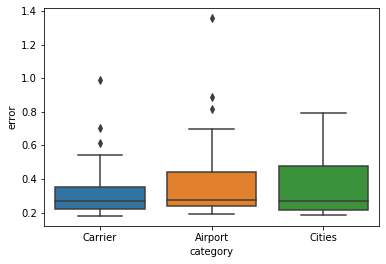
\includegraphics[width=0.6\textwidth, height=0.24\textheight]{./img/cats_arrdelay.png}
  \centering
  \caption{
  Distribución de errores promedio en predicción de delay de arribos (en minutos) sobre 4 splits de cross-validation para cada entidad del top5 de cada categoría.
  }
  \label{fig:cats-arrdelay}
\end{figure}

\begin{figure}[h]
  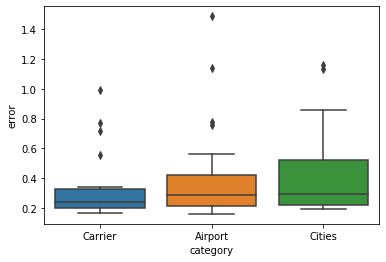
\includegraphics[width=0.6\textwidth, height=0.24\textheight]{./img/cats_depdelay.png}
  \centering
  \caption{
  Distribución de errores promedio en predicción de delay de partidas (en minutos) sobre 4 splits de cross-validation para cada entidad del top 5 de cada categoría.
}
  \label{fig:cats-depdelay}
\end{figure}
\subsubsection{El 9/11 y el impacto en predicciones de OTP}
%  que paso el 9/11 y como se esperaria que afecte, que medidas de seguridad
%   pudieron haber tomado
%  rangos que tomamos y que resultados dieron
Otra pregunta que nos hicimos fue cómo afectó, a través de la reacción en términos de políticas y rigor aeroportario, el atentado del 9/11 en Estados Unidos a las predicciones sobre delay. Consideramos por un lado que podría ser posible ver aumentos en delay por cuestiones de mayores exigencias de seguridad antes de salir a pista, o sino ver un decrecimiento en delays provocado por mayor planificación en respuesta, en ambos casos generando errores de predicción.

\begin{figure}[h]
  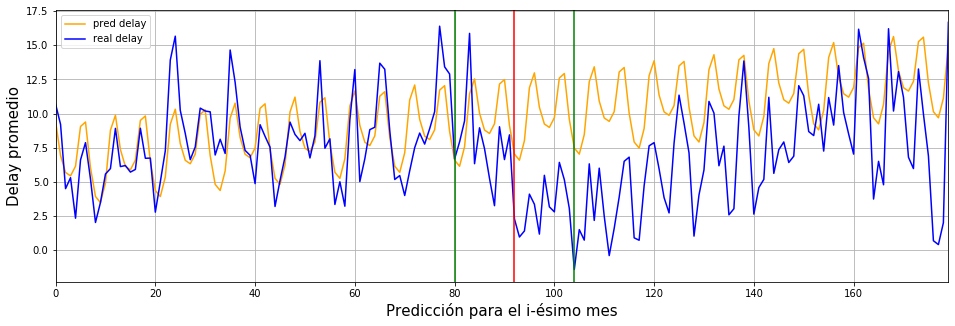
\includegraphics[width=1.0\textwidth, height=0.24\textheight]{./img/nine_eleven.png}
  \centering
  \caption{
  Predicción de delay en minutos contra delay histórico. Las líneas verdes marcan el intervalo de predicción sobre el cual se considera el error antes y despues del atentando, representado por la línea roja.
}
  \label{fig:nine_eleven}
\end{figure}

Para experimentar entrenamos al predictor de CML con datos anteriores a un año antes del atentado y comparamos el NMSE de las predicciones antes del atentado contra un año después del mencionado. En predicciones diarias notamos una diferencia entre aproximadamente 0.11 y 0.17 de RMSE antes y después del atentado respectivamente mientras que la diferencia en predicciones mensuales resultó de 0.28 y 1.26, con lo que resultaría que el impacto a nivel predicciones es importante (como se puede apreciar en la figura \ref{fig:nine_eleven}). Indagando más profundo descubrimos que el promedio de delay pasó de al rededor de 8 minutos antes del atentado a 3 luego de este, validando la hipótesis de una mayor planificación.

\subsection{Segundo eje de experimentación}
En el segundo eje intentamos contemplar otros factores de impacto que no hayamos considerado originalmente para el primero.
\subsubsection{Demoras en el arribo causados por demoras en los despegues}%
\label{sub:dep_arr_delay}

Es razonable pensar que un vuelo que se demora al despegar, va a demorarse
también al aterrizar. Se estudió la correlación entre la demora al despegue,
\texttt{DepDelay} y la demora en el momento del aterrizaje \texttt{ArrDelay}.
Se obtuvo una correlación alta, de $\rho=0.92$.

Para limpiar los datos, se utilizó un filtro de \textit{outliers} basado en una
regla escrita a mano que descarta los vuelos que se adelantan varias horas a su
hora de despegue programada. Creemos que se tratan de errores de medición.

\begin{figure}[h]
\centering
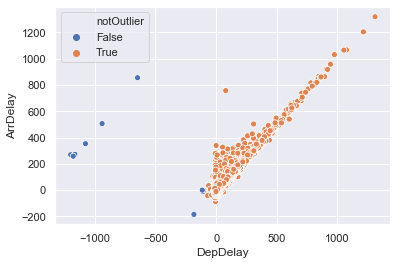
\includegraphics[width=0.5\textwidth]{img/dep_arr_delay_outliers_a_mano.png}
\caption{Relación entre la demora al despegar y la demora al aterrizar.}
\end{figure}

Finalmente, se entrenó un modelo de regresión lineal entre ambas variables obteniendo un \textsc{nrmse} de $0.00646$.
La mayor densidad de puntos se encuentra sobre la
recta del modelo.
Por otro lado, en el rango de $-200 \leq \mathrm{DepDelay} \leq 800$ pueden observarse vuelos con un mayor
\textit{delay} al predicho por el modelo. Se propone para un futuro
experimento, añadir regresores adicionales para mejorar la predicción en dicha zona.

\begin{figure}[h]
\centering
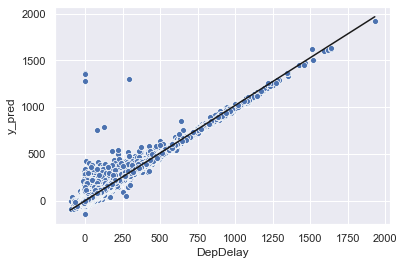
\includegraphics[width=0.5\textwidth]{img/dep_arr_delay_regplot.png}
\caption{Regresión lineal entre la demora al despegar y la demora al aterrizar.}
\end{figure}

\begin{figure}[h]
\centering
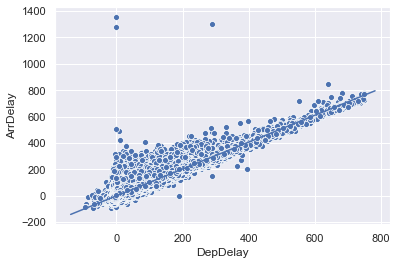
\includegraphics[width=0.5\textwidth]{img/dep_arr_delay_detalle.png}
\caption{
    Detalle de la regresión lineal para la demora al despegar y la demora al
    aterrizar en el rango $-200 \leq \mathrm{DepDelay} \leq 800$.
}
\end{figure}

\subsubsection{Demoras de arribos y Cancelaciones}

Otro eje interesante es el de usar la cantidad de cancelaciones como
KPI. Se hipotetizó una relación dinámica entre las demoras y las
cancelaciones, ya que ambas pueden influirse mutuamente.

Para el análisis se agregaron los datos de todo el dataset por día
obviandose los datos del 2001, que presentan características propias
por la situación política y de seguridad.

Se eliminaron del dataset todas las cancelaciones debidas a factores
climáticos y de razones de seguridad, para disminuir el peso de
factores ajenos a la calidad del servicio.

\begin{figure}[h]
  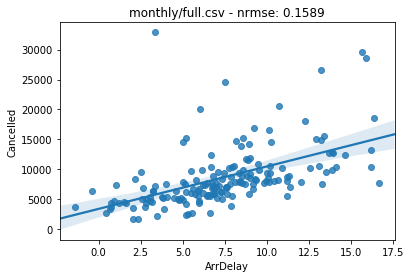
\includegraphics[width=0.6\textwidth, height=0.24\textheight]{./img/arrDel_vs_cancell.png}
  \centering
  \caption{ Relación entre las demoras de arribo y las cancelaciones,
    para todo el dataset desde 1994 hasta 2008 sin incluir 2001. Los
    datos están agregados por día. Las cancelaciones se sumaron, las
    demoras se promediaron.  }
  \label{fig:cancell-arrdelay}
\end{figure}

En la figura \ref{fig:cancell-arrdelay}, vemos una buena correlación
entre ambas variables con un \emph{nrmse} que si bien no es
despreciable, nos permite establecer una correlación lineal.

También nos preguntamos si las demoras o las cancelaciones, podían
afectar periodos posteriores. Para esto generamos una matriz de
correlación, para los mismos datos anteriores, tomando las
cancelaciones del día actual vs la demora y también las cancelaciones
de dos días en el futuro y en el pasado. En la figura
\ref{fig:cancell-arrdelay}. Se ve que la mayor correlación se
encuentran entre días concecutivos para las cancelaciones, incluso
superando la alta correlación entre demora y cancelaciones del día
actual mostradas en la fig. \ref{fig:cancell-arrdelay} \footnote{Las
  métricas no son iguales en ambas figuras.}

\begin{figure}[h]
  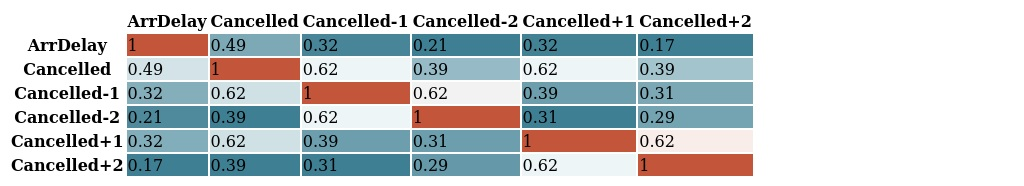
\includegraphics[width=0.6\textwidth, height=0.24\textheight]{./img/daily-full-csv-correlation-table.jpg}
  \centering
  \caption{ Correlacion entre las demoras de arribo y las
    cancelaciones para días cercanos. Las cancelaciones están
    shiteadas hacía adelante y hacía atrás. Los datos se tomaron para
    todo el dataset desde 1994 hasta 2008 sin incluir 2001. Los datos
    están agregados por día. Las cancelaciones se sumaron, las demoras
    se promediaron.  }
  \label{fig:cancell-arrdelay}
\end{figure}


\section{Referencias}

\bibliographystyle{plain}
\bibliography{bibliography.bib}

\end{document}
